\documentclass{assignment}

\course{ECO 120-04}
\name{Lucas Reddinger}
\date{Monday 26 September 2022}
\doctitle{Assignment 2 Solutions}

\begin{document}
\RaggedRight

\beginsolutions{}

\section{An economy of kale and dental floss}

Your small country produces two goods, kale and dental floss.

When production is efficient, you can produce the following combinations of kale and dental floss:

{\footnotesize \begin{tabular}{l>{\raggedleft\arraybackslash}p{0.9in}>{\raggedleft\arraybackslash}p{1.3in}}
\toprule
Point & Kale (tons) & Dental floss (km) \\
\midrule
$A$ &   0 & 1,000 \\
$B$ & 200 &   900 \\
$C$ & 400 &   700 \\
$D$ & 600 &   400 \\
$E$ & 800 &     0 \\
\bottomrule
\end{tabular} }

These points are connected with straight line segments; altogether these comprise the production possibility frontier.

\begin{enumerate}

\item Please graph the production possibility frontier (PPF), with kale on the horizontal axis and dental floss on the vertical axis. Use a scale of 0 to 1,200 on the horizontal axis and 0 to 1,000 on the vertical axis. Properly label the graph by labelling both the axes and the curve.

\begin{solution}
\begin{center}

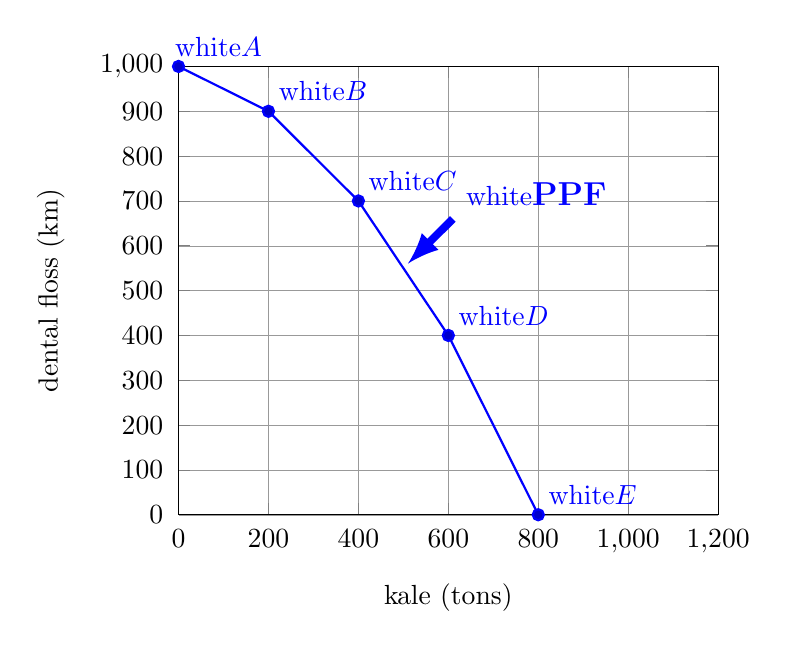
\begin{tikzpicture}[scale=1, x=4mm, y=4mm, >=latex]
\begin{axis}[
  grid=both,
  grid style={line width=.1pt, draw=black!40!white},
  xmin=0,
  ymin=0,
  xmax=1200,
  ymax=1000,
  xtick distance=200,
  ytick distance=100,
  xlabel={kale (tons)},
  ylabel={dental floss (km)},
  xticklabel style={yshift=-2pt},
  yticklabel style={xshift=-2pt},
  xlabel style={yshift=-4pt},
  ylabel style={yshift=6pt}
]

\addplot+ [
  mark=*, thick,
  visualization depends on=\thisrow{xshift} \as \xshift,
  point meta=explicit symbolic,
  nodes near coords,
  every node near coord/.style={above right, xshift=\xshift}
] table [meta=label,meta index=xshift] {
x y label xshift
    0   1000 \contour{white}{$A$} -5
    200  900 \contour{white}{$B$}  0
    400  700 \contour{white}{$C$}  0
    600  400 \contour{white}{$D$}  0
    800    0 \contour{white}{$E$}  0
};

\draw[blue,line width=1mm,<-](axis cs:  510, 560)--++(axis cs:  100, 100) node[above right,blue]{\contour{white}{\textbf{\large PPF}}};
\end{axis}
\end{tikzpicture}

\end{center}
\end{solution}

\item The PPF you drew above should consist of four line segments---$\overline{AB}$, $\overline{BC}$, $\overline{CD}$, and $\overline{DE}$. For each segment, please calculate the cost of one ton of kale. Ensure that you specify the units of the cost. Please show your work. If you use a formula, please write it clearly upon its first use.
\begin{solution}
\vspace{-\baselineskip}
\begin{align*}
\text{Slope:} &&& \frac{\text{change in $y$}}{\text{change in $x$}} \\
\text{Slope of $\overline{AB}$:} &&& \frac{(900-1000)\text{ km floss}}{(200-0)\text{ tons kale}} = \frac{-100\text{ km floss}}{200\text{ tons kale}} = -1/2 \text{ km floss per ton kale} \\
\text{Slope of $\overline{BC}$:} &&& \frac{-200\text{ km floss}}{200\text{ tons kale}} = -1 \text{ km floss per ton kale} \\
\text{Slope of $\overline{CD}$:} &&& \frac{-300\text{ km floss}}{200\text{ tons kale}} = -3/2 \text{ km floss per ton kale} \\
\text{Slope of $\overline{DE}$:} &&& \frac{-400\text{ km floss}}{200\text{ tons kale}} = -2 \text{ km floss per ton kale}
\end{align*}
\end{solution}

\item Now for each segment, please calculate the cost of one kilometer of dental floss. Again, please show your work and ensure that you specify the units of the cost.
\begin{solution}
\vspace{-\baselineskip}
\begin{align*}
\text{Inverse slope:} &&& \frac{\text{change in $x$}}{\text{change in $y$}} \\
\text{Inverse slope of $\overline{AB}$:} &&& \frac{(200-0)\text{ tons kale}}{(900-1000)\text{ km floss}} = \frac{200\text{ tons kale}}{-100\text{ km floss}} = -2 \text{ tons kale per km floss} \\
\text{Inverse slope of $\overline{BC}$:} &&& \frac{200\text{ tons kale}}{-200\text{ km floss}} = -1 \text{ ton kale per km floss} \\
\text{Inverse slope of $\overline{CD}$:} &&& \frac{200\text{ tons kale}}{-300\text{ km floss}} = -2/3 \text{ tons kale per km floss} \\
\text{Inverse slope of $\overline{DE}$:} &&& \frac{200\text{ tons kale}}{-400\text{ km floss}} = -1/2 \text{ tons kale per km floss}
\end{align*}
\end{solution}

\item What is the cost of the 500th ton of kale? Please specify units.

\begin{solution}
The 500th ton of kale---meaning the 1 ton that we produce last, following production of 499 tons of kale---is on the $\overline{CD}$ segment, so it costs $3/2$ (or $1.5$) km of dental floss.
\end{solution}

\item What is the cost of the 921st km of dental floss? Please specify units.

\begin{solution}
The 921st km of dental floss---meaning the 1 km that we produce last, following production of 920 km of dental floss---is on the $\overline{AB}$ segment, so it costs $2$ tons of kale.
\end{solution}

\end{enumerate}

\clearpage

\section{Technological progress}

New irrigation technology allows you to produce more kale. Now efficient production is given by the following table:

\begin{tabular}{l>{\raggedleft\arraybackslash}p{0.9in}>{\raggedleft\arraybackslash}p{1.3in}}
\toprule
Point & Kale (tons) & Dental floss (km) \\
\midrule
$A'$ &     0 & 1,000 \\
$B'$ &   300 &   900 \\
$C'$ &   600 &   700 \\
$D'$ &   900 &   400 \\
$E'$ & 1,200 &     0 \\
\bottomrule
\end{tabular}

Once again, these points are connected with straight line segments, comprising the new PPF.

\begin{enumerate}

\item Please draw this new PPF on your original graph, labeled as PPF'.

\begin{solution}
\begin{center}
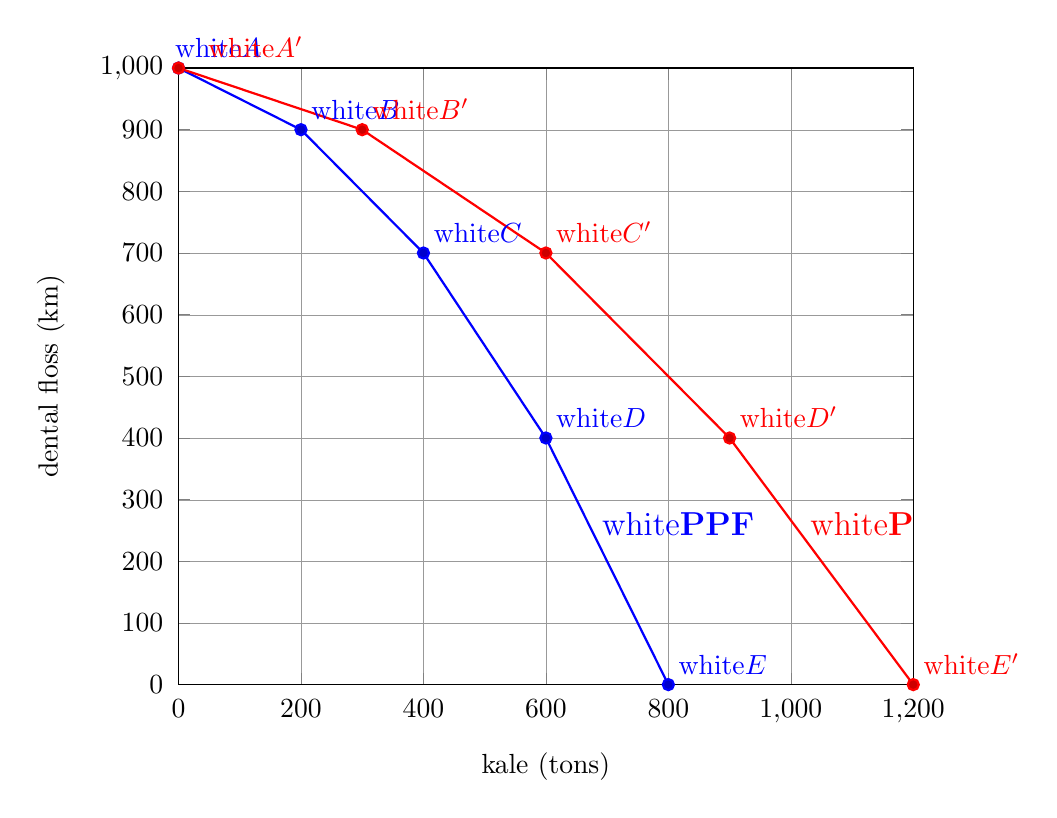
\begin{tikzpicture}[x=4mm, y=4mm, >=latex]
\begin{axis}[
  width={0.9\linewidth},
  grid=both,
  grid style={line width=.1pt, draw=black!40!white},
  xmin=0,
  ymin=0,
  xmax=1200,
  ymax=1000,
  xtick distance=200,
  ytick distance=100,
  xlabel={kale (tons)},
  ylabel={dental floss (km)},
  xticklabel style={yshift=-2pt},
  yticklabel style={xshift=-2pt},
  xlabel style={yshift=-4pt},
  ylabel style={yshift=6pt}
]

\addplot+ [
  mark=*, thick,
  visualization depends on=\thisrow{xshift} \as \xshift,
  point meta=explicit symbolic,
  nodes near coords,
  every node near coord/.style={above right, xshift=\xshift}
] table [meta=label,meta index=xshift] {
x y label xshift
0   1000 \contour{white}{$A$} -5
200  900 \contour{white}{$B$}  0
400  700 \contour{white}{$C$}  0
600  400 \contour{white}{$D$}  0
800    0 \contour{white}{$E$}  0
};

\addplot+ [
  mark=*, thick,
  visualization depends on=\thisrow{xshift} \as \xshift,
  point meta=explicit symbolic,
  nodes near coords,
  every node near coord/.style={above right, xshift=\xshift}
] table [meta=label,meta index=xshift] {
x y label xshift
0   1000 \contour{white}{$A'$} 7
300  900 \contour{white}{$B'$} 0
600  700 \contour{white}{$C'$} 0
900  400 \contour{white}{$D'$} 0
1200   0 \contour{white}{$E'$} 0
};

\node[label={[font=\large,text=blue]0:{\contour{white}{\textbf{PPF}}}}] at (axis cs:  660, 260) {};
\node[label={[font=\large,text=red]0:{\contour{white}{\textbf{PPF'}}}}] at (axis cs:  1000, 260) {};
\end{axis}
\end{tikzpicture}

\end{center}
\end{solution}

\clearpage

\item With your new irrigation technology, what is the cost of the 500th ton of kale? Please show your work and specify units.

\begin{solution}
\emph{Complete answer:} The 500th ton of kale costs 2/3 km of dental floss.

$$\text{Slope of $\overline{B'C'}$:} \quad \frac{-200\text{ km floss}}{300\text{ tons kale}} = -2/3 \text{ km floss per ton kale}.$$

Thus the 500th ton of kale---meaning the 1 ton that we produce last, following production of 499 tons of kale---costs 2/3 km of dental floss.
\end{solution}

Did the cost increase, decrease, or remain the same compared to the cost with the old technology?

\begin{solution}
\emph{Complete answer:} The cost of kale has decreased.

The 500th ton of kale previously cost $3/2=1.5$ km of dental floss; it now costs only $2/3\approx0.67$ km of dental floss. Thus the cost has decreased. Because kale productivity increased, each ton of kale now costs less dental floss.
\end{solution}

\item With your new irrigation technology, what is the cost of the 921st km of dental floss? Please show your work and specify units.

\begin{solution}
\emph{Complete answer:} The 921st km of dental floss costs 3 tons of kale.

$$\text{Slope of $\overline{A'B'}$:} \quad \frac{300\text{ tons kale}}{-100\text{ km floss}} = -3 \text{ tons kale per km floss}.$$

Thus the 921st km of dental floss---meaning the 1 km that we produce last, following production of 920 km of dental floss---costs 3 tons of kale.
\end{solution}

Did the cost increase, decrease, or remain the same compared to the cost with the old technology?

\begin{solution}
\emph{Complete answer:} The cost of dental floss has increased.

The 921st km of dental floss previously cost 2 tons of kale; it now costs 3 tons of kale. Thus the cost has increased. Because kale productivity increased, additional kale is forgone when we produce dental floss, compared to the old technology. Thus the cost of dental floss has increased.
\end{solution}

\end{enumerate}

\end{document}
